% [12pt,a4paper,bibliography=totocnumbered,listof=totocnumbered]{scrartcl}
\documentclass[12pt,a4paper]{article}
\usepackage{mathtools}
\usepackage[ngerman]{babel}
\usepackage[utf8]{inputenc}
\usepackage{amsmath}
\usepackage{amsfonts}
\usepackage{amssymb}
\usepackage{graphicx}
\usepackage{fancyhdr}
\usepackage{tabularx}
\usepackage{geometry}
\usepackage{setspace}
\usepackage[right]{eurosym}
\usepackage[printonlyused]{acronym}
\usepackage{subfig}
\usepackage{floatflt}
\usepackage{float}
\usepackage[usenames,dvipsnames]{color}
\usepackage{colortbl}
\usepackage{paralist}
\usepackage{array}
\usepackage{titlesec}
\usepackage{parskip}
\usepackage[right]{eurosym}
%\usepackage{picins}
\usepackage[subfigure,titles]{tocloft}
\usepackage[pdfpagelabels=true]{hyperref}

\usepackage{listings}

%\usepackage[
%backend=biber,
%style=alphabetic-verb,
%citestyle=alphabetic-verb
%]{biblatex}
%\usepackage{biblatex} 
%\addbibresource{literatur.bib}


\lstset{basicstyle=\ttfamily\tiny, captionpos=b, breaklines=true, showstringspaces=false, tabsize=2, xleftmargin=0em, framexleftmargin=0em}
\makeatletter
\def\l@lstlisting#1#2{\@dottedtocline{1}{0em}{1em}{\hspace{1,5em} Lst. #1}{#2}}
\makeatother

\geometry{a4paper, top=27mm, left=20mm, right=20mm, bottom=35mm, headsep=10mm, footskip=12mm}


\hypersetup{unicode=false, pdftoolbar=true, pdfmenubar=true, pdffitwindow=false, pdfstartview={FitH},
	pdftitle={Wahlpflichtfach: Implementierung von Brettspielen am Beispiel ReversiXT (SS \the\year)},
	pdfauthor={Dr.\ Carsten Kern},
	pdfsubject={Projektbericht},
	pdfcreator={\LaTeX\ with package \flqq hyperref\frqq},
	pdfproducer={pdfTeX \the\pdftexversion.\pdftexrevision},
	pdfkeywords={Projektbericht, ReversiXT},
	pdfnewwindow=true,
	colorlinks=true,linkcolor=black,citecolor=black,filecolor=magenta,urlcolor=black}
\pdfinfo{/CreationDate (D:20151500000000)}

\begin{document}
\titlespacing{\section}{0pt}{12pt plus 4pt minus 2pt}{-6pt plus 2pt minus 2pt}

% Kopf- und Fusszeile
\renewcommand{\sectionmark}[1]{\markright{#1}}
\renewcommand{\leftmark}{\rightmark}
\pagestyle{fancy}
\lhead{}
\chead{}
\rhead{\thesection\space\contentsname}
\lfoot{Implementierung von Brettspielen am Beispiel ReversiXT -- SS \the\year}
\cfoot{}
\rfoot{\ \linebreak Seite \thepage}
\renewcommand{\headrulewidth}{0.4pt}
\renewcommand{\footrulewidth}{0.4pt}

% Vorspann
\renewcommand{\thesection}{\Roman{section}}
\renewcommand{\theHsection}{\Roman{section}}
\pagenumbering{Roman}

\newcommand{\folgen}[1]{
\ensuremath
#1
}

\newcommand{\MyTitlepage}[5][\empty]{
\thispagestyle{empty}
\begin{center}
	
\includegraphics[scale=0.2]{pics/oth-logo.png}\\
	\vspace*{2cm}
	\Large
	\textbf{Fakultät}\\
	\textbf{Informatik und Mathematik}\\
	\vspace*{2cm}
	\Huge
	\textbf{Projektbericht}\\
	\vspace*{0.5cm}
	\large
	zum HSP1 im Wintersemester 2019/20\\
	\vspace*{1cm}
	\textbf{Implementierung von Reversi mit dem AlphaZero-Ansatz}\\
	\vspace*{1cm}
	%\includegraphics[height=6cm]{#1}
	\vfill
	\normalsize
	%\newcolumntype{x}[1]{>{\raggedleft\arraybackslash\hspace{0pt}}p{#1}}
	\begin{tabular}{rl}%{6cm}p{7.5cm}}
		\rule{0mm}{5ex}\textbf{Autoren:} & \hspace*{-0.5em}\begin{tabular}[t]{r}#3\end{tabular} \\ 
		\rule{0mm}{5ex}\textbf{Leiter:} & Prof. Dr. rer. nat. Carsten Kern \\ 
		\rule{0mm}{5ex}\textbf{Abgabedatum:} & #4 \\ 
	\end{tabular} 
\end{center}
\pagebreak
}


% ----------------------------------------------------------------------------------------------------------
% Titelseite
% ----------------------------------------------------------------------------------------------------------
\MyTitlepage{}{
\texttt{simon1.hofmeister@st.oth-regensburg.de}\\
\texttt{nadiia1.matsko@st.oth-regensburg.de}\\
\texttt{monika.silber@st.oth-regensburg.de}\\
\texttt{simon.wasserburger@st.oth-regensburg.de}}
{15.03.\the\year}

\setcounter{page}{1} 
% ----------------------------------------------------------------------------------------------------------
% Inhaltsverzeichnis
% ----------------------------------------------------------------------------------------------------------
\tableofcontents
\pagebreak


% ----------------------------------------------------------------------------------------------------------
% Inhalt
% ----------------------------------------------------------------------------------------------------------
% Abstände Überschrift
\titlespacing{\section}{0pt}{12pt plus 4pt minus 2pt}{-6pt plus 2pt minus 2pt}
\titlespacing{\subsection}{0pt}{12pt plus 4pt minus 2pt}{-6pt plus 2pt minus 2pt}
\titlespacing{\subsubsection}{0pt}{12pt plus 4pt minus 2pt}{-6pt plus 2pt minus 2pt}

% Kopfzeile
\renewcommand{\sectionmark}[1]{\markright{#1}}
\renewcommand{\subsectionmark}[1]{}
\renewcommand{\subsubsectionmark}[1]{}
\lhead{Kapitel \thesection}
\rhead{\rightmark}

\onehalfspacing
\renewcommand{\thesection}{\arabic{section}}
\renewcommand{\theHsection}{\arabic{section}}
\setcounter{section}{0}
\pagenumbering{arabic}
\setcounter{page}{1}

% ----------------------------------------------------------------------------------
% Kapitel: Einleitung
% ----------------------------------------------------------------------------------

\section{Einleitung}
Das Ziel des vorliegenden Projektes ist es das Spiel \glqq{}Reversi\grqq{} mithilfe von Methoden aus dem Bereich der künstlichen Intelligenz zu implementieren. Dazu wird der entsprechende Reinforcement-Learning-Ansatz von AlphaZero beziehungsweise AlphaGo Zero angewendet, der ein neuronales Netz in Kombination mit dem Monte-Carlo-Suchverfahren nutzt.

\subsection{Reversi}

In diesem Abschnitt werden die grundlegenden Spielregeln\footnote{$https://de.wikipedia.org/wiki/Othello_(Spiel)$} von Reversi, so wie sie ebenfalls im vorliegenden Projekt Anwendung finden, vorgestellt.

%TODO Anzahl Spieler, Startzustand, Aussetzen (nur wenn man keinen Zug machen kann?)
Reversi ist ein kompetitives Spiel, bei dem die Teilnehmer in einer vorgegebenen Reihenfolge Züge machen dürfen. Bei zwei Spielern bedeutet das, dass sich diese abwechseln, bei mehr als zwei geht es reihum. Jeder Spieler hat eine Farbe beziehungsweise ein Symbol für seine gelegten Steine. Ein Zug besteht darin, den eigenen Spielstein angrenzend an einen gegnerischen Stein so auf dem Spielfeld zu platzieren, dass mindestens ein gegnerischer eingeschlossen wird, wobei es stattdessen außerdem möglich ist auszusetzen. Sobald der eigene Spielstein positioniert ist, werden alle gegnerischen, die zwischen dem neuen und bereits vorhandenen Steinen liegen, so umgekehrt, dass sie die Farbe oder das Symbol des derzeitigen Spielers annehmen.

Üblicherweise ist das Spielfeld ein Quadrat der Größe 8x8, wobei in Abwandlungen andere Dimensionen grundsätzlich möglich sind. Ein typischer Startzustand zeigt dich darin, dass bereits zwei Steine der beiden Spieler, also ingesamt vier, in der Mitte des Feldes in Form einer 2x2 Anordnung platziert sind. Die Steine der jeweiligen Teilnehmer sind dabei diagonal angeordnet.

Ziel ist es, möglichst viele Steine der eigenen Farbe oder mit dem eigenen Symbol auf dem Feld zu haben. Das Spiel ist beendet, sobald beide Spieler direkt hintereinander passen beziehungsweise beide keine Züge mehr machen können. Gewonnen hat entsprechend derjenige, der mehr Spielsteine auf dem Feld liegen hat. Falls beide Teilnehmer die gleiche Anzahl haben, so ist der Spielausgang unentschieden.

%TODO XT bzw. Erweiterungen
\subsection{ReversiXT}
\subsection{AlphaGo}
AlphaGo ist ein Computerprogramm, das das Brettspiel Go spielt\cite{BBC_NewsGo}. Es wurde von DeepMind Technologies entwickelt, das später von Google übernommen wurde. AlphaGo hatte drei weitaus mächtigere Nachfolger, genannt AlphaGo Master, AlphaGo Zero und AlphaZero \cite{DeepMind}.

Im März 2016 schlug AlphaGo Lee Sedol in einem Fünf-Spiel-Match, das erste Mal, dass ein Computer-Go-Programm einen 9-Dan-Profi ohne Handicap besiegte \cite{AlphaGoMatch}. Obwohl es im vierten Spiel gegen Lee Sedol verlor, trat Lee im Endspiel zurück und gab im Endergebnis 4 zu 1 zu Gunsten von AlphaGo. In Anerkennung des Sieges wurde AlphaGo von der Korea Baduk Association mit einem Ehren-9-Dan ausgezeichnet \cite{AlphaGoDan}. Der Vorsprung und das Herausforderungsspiel mit Lee Sedol wurden in einem Dokumentarfilm mit dem Titel AlphaGo, \cite{AlphaGoFilm} unter der Regie von Greg Kohs dokumentiert. Er wurde am 22. Dezember 2016 von Science als einer der zweiten Durchbruch des Jahres gewählt \cite{Science2016}.

AlphaGo und seine Nachfolger verwenden einen Monte Carlo Baumsuch-Algorithmus, um seine Züge auf der Grundlage von Wissen zu finden, das zuvor durch maschinelles Lernen "gelernt" wurde, insbesondere durch ein künstliches neuronales Netz (eine deep learning Methode) durch ausführliches Training, sowohl durch menschliches als auch durch Computerspiel \cite{Silver_2016}. Ein neuronales Netz wird trainiert, um AlphaGos eigene Zugauswahlen und auch die Partien der Gewinner vorherzusagen. Dieses neuronale Netz verbessert die Stärke der Baumsuche, was zu einer höheren Qualität der Zugauswahl und einem stärkeren Selbstspiel in der nächsten Iteration führt.

\textbf{AlphaGo Spielstil}

Im Spiel gegen einen Top-Go-Spieler, hat das künstliche Intelligenzprogramm AlphaGo die Kommentatoren mit Zügen verwirrt, die oft als \glqq schön\grqq{} beschrieben werden, aber nicht in den üblichen menschlichen Spielstil passen \cite{Ribeiro2016}.


Howard Yu,Professor für strategisches Management und Innovation an der IMD Business School meinte, dass AlphaGo  eine Maschine darstellt, die nicht nur denkt, sondern auch lernen und Strategien entwickeln kann \cite{Ribeiro2016}.

Toby Manning, der Match-Schiedsrichter für AlphaGo vs. Fan Hui, hat den Stil des Programms als "konservativ" beschrieben \cite{Gibney2016}. Der Spielstil von AlphaGo begünstigt stark die größere Wahrscheinlichkeit, mit weniger Punkten zu gewinnen, gegenüber der geringeren Wahrscheinlichkeit, mit mehr Punkten zu gewinnen \cite{Ribeiro2016}. Seine Strategie, die Gewinnwahrscheinlichkeit zu maximieren, unterscheidet sich von dem, wozu menschliche Spieler neigen, nämlich territoriale Gewinne zu maximieren, und erklärt einige seiner seltsam aussehenden Züge \cite{Chouard2016}.


\subsection{AlphaZero}
AlphaZero ist ein Computerprogramm, das von der Forschungsfirma \textit{DeepMind} für künstliche Intelligenz entwickelt wurde, um die Spiele Schach, Shogi und Go zu meistern. Der Algorithmus verwendet einen ähnlichen Ansatz wie AlphaGo Zero \cite{SilverHubert2017}. 


Das neuronale Netz von AlphaGo Zero weiß nichts über das Spiel jenseits der Regeln. Im Gegensatz zu früheren Versionen von AlphaGo nahm AlphaGo Zero nur die Steine des Bretts wahr, anstatt einige seltene, vom Menschen programmierte Randfälle zu haben, die helfen, ungewöhnliche Go-Brettstellungen zu erkennen. Die KI beschäftigte sich mit dem Reinforcement Learning und spielte gegen sich selbst, bis sie ihre eigenen Züge und deren Auswirkungen auf den Ausgang des Spiels vorhersehen konnte \cite{Greenemeier2017}.


AlphaZero ersetzt das handgemachte Wissen und die domänenspezifischen Erweiterungen, die in traditionellen Spielprogrammen verwendet werden, durch tiefe neuronale Netze, einen universellen Reinforcement Learning-Algorithmus und einen universellen Baumsuch-Algorithmus \cite{Silver2018}. 
Statt einer handgemachten Auswertungsfunktion und Heuristik für die Zugreihenfolge verwendet AlphaZero ein tiefes neuronales Netzwerk. Die Parameter des tiefen neuronalen Netzes in AlphaZero werden durch Reinforcement Learning trainiert indem AlphaZero mit sich selber spielt und Parameter zufällig initialisiert. Statt einer Alpha-Beta-Suche mit domänenspezifischen Erweiterungen verwendet AlphaZero einen universellen Monte-Carlo-Baumsuch-Algorithmus \cite{Silver2018}. AlphaZero ist eine verallgemeinerte Variante des AlphaGo Zero Algorithmus und kann neben Go auch Shogi und Schach spielen. Die Unterschiede zwischen AlphaZero und AlphaGo Zero sind: \cite{Silver2018}
\begin{enumerate}
	\item AZ hat fest programmierte Regeln für die Einstellung von Such-Hyperparametern.
	\item Das neuronale Netz wird nun ständig aktualisiert.
	\item Go ist (im Gegensatz zu Schach) unter bestimmten Reflexionen und Rotationen symmetrisch; AlphaGo Zero wurde programmiert, um diese Symmetrien auszunutzen. AlphaZero ist es nicht.
	\item Schach kann im Gegensatz zu Go mit einem Unentschieden enden; daher kann AlphaZero die Möglichkeit einer unentschiedenen Partie in Betracht ziehen.
\end{enumerate}
Im Jahr 2019 veröffentlichte DeepMind ein neues Artikel über MuZero, einen neuen Algorithmus, der in der Lage ist, auf AlphaZero Arbeit zu verallgemeinern, indem er sowohl Atari als auch Brettspiele ohne Kenntnis der Regeln oder Darstellungen des Spiels spielt \cite{Silver_2019}. 





%In den ersten drei Tagen spielte AlphaGo Zero 4,9 Millionen Spiele gegen sich selbst in schneller Folge \cite{Kennedy2017}. Es schien die Fähigkeiten zu entwickeln, die erforderlich waren, um Spitzenleute innerhalb weniger Tage zu schlagen, während das frühere AlphaGo Monate des Trainings benötigte, um das gleiche Niveau zu erreichen \cite{Klein2017}.


%Am 5. Dezember 2017 veröffentlichte das DeepMind-Team einen Vorabdruck, der AlphaZero vorstellte, das innerhalb von 24 Stunden ein übermenschliches Spielniveau in diesen drei Partien erreichte, indem es die Weltmeisterprogramme Stockfish, elmo und die 3-Tage-Version von AlphaGo Zero besiegte. In jedem dieser Spiele wurden spezielle Tensor Processing Units (TPUs) verwendet, für deren Verwendung die Google-Programme optimiert wurden \cite{SilverHubert2017}.  DeepMind's Arbeit über AlphaZero wurde am 7. Dezember 2018 in der Zeitschrift Science veröffentlicht.

 


\newpage

% ----------------------------------------------------------------------------------
% Kapitel: Related Work/Theorie
% ----------------------------------------------------------------------------------
\section{Theoretische Grundlagen}

\subsection{Monte Carlo Tree Search}
Der MCTS findet als Alternative zum Alpha-Beta-Search Anwendung. Da der Alpha-Beta-Ansatz einen geringen Verzweigungsgrad und eine angemessene Bewertungsfunktion fordert, ist dessen in Anwendung in Brettspielen, die diese Bedingungen nicht erfüllen, ungeeignet. Der MCTS hingegen bewies sich im Umgang mit solchen Situation \cite{Chaslot2008}.
Basierend auf einer Bestensuche und stochastischer Simulation  wählt der MCTS bei jedem Durchlauf den erfolgversprechendsten Knoten als nächsten Spielzug aus. Entsprechend wird ein Baum aufgebaut, in dem ein Knoten einen konkreten Spielzustand widerspiegelt\cite{Chaslot2008}. Dabei werden die drei Schritte Expansion, Simulation und Backpropagation durchgeführt \cite{Chaslot2008}. Falls der aktuelle Spielzustand noch nicht als Knoten existiert, wird der Baum zunächst expandiert. Um nun die beste Aktion zu ermitteln, werden Spiele ausgehend vom aktuellen Zustand bis hin zum Spielende simuliert. Dabei werden valide Spielzüge zufällig ausgewählt. Hierbei ist jedoch zu beachten, dass eine reine Zufallsauswahl, die impliziert, dass die Selektion aller Möglichkeiten gleich wahrscheinlich ist, in eher primitivem Spielverhalten resultiert. Mithilfe einer Heuristik können daher aussichtsreichere Spielzüge favorisiert werden. Innerhalb eines Playouts durchlaufene Nodes werden schließlich aktualisiert, indem vermerkt wird, dass sie einmal mehr besucht wurden und welches Spielergebnis sich ergeben hat \cite{Chaslot2008}. 

Anzumerken ist, dass zwei verschiedene Policies genutzt werden. Für die Erweiterung des Baums wird eine Tree Policy angewendet, die besagt, dass entsprechende Blattknoten an bereits vorhandene, unbesuchte Knoten angefügt werden. Des Weiteren legt die Default Policy die Simulation fest. Hierbei wird in einem nichtterminalen Spielzustand, der gewöhnlich dem neu hinzugefügt Blattknoten entspricht, ein zufälliges Spiel durchlaufen, um ein ein Spielergebnis zu ermitteln \cite{Browne2012}. 

Der MCTS bleibt so lange aktiv, bis er unterbrochen wird, beispielsweise aufgrund von abgelaufener Rechenzeit. Der zu diesem Zeitpunkt als am erfolgreichsten ermittelte Knoten beziehungsweise Spielzug steht daraufhin fest \cite{Browne2012}.

Zu einem Knoten gehören der entsprechende Spielzustand, den er widerspiegelt, der Spielzug aus dem er resultierte, sowie der aus Simulationen resultierende Reward und wie oft er besucht wurde \cite{Browne2012}.

Nachfolgend werden die konkreten Umsetzungsdetails des MCTS in AlphaGo Zero betrachtet, so wie sie von Silver et al. angewendet wurden \cite{Silver2017}.
In AlphaGo Zero besteht der Selection-Schritt daraus, ausgehend von einem Wurzelknoten eine Simulationen bis hin zu einem Blattknoten zu durchlaufen. Dafür wird in jedem Schritt der Folgeknoten ausgewählt, der den maximalen UCT-Wert enthält \cite{Silver2017}.

Entsprechend dem AlphaZero-Ansatz findet bei der Simulation keine zufällige Auswahl des Spielzuges statt, stattdessen wird eine Variante des Upper Confidence Bound (UCB) angewendet. Die konkrete Abwandlung ist der polynomiale UCB applied to Trees (UCT). Dieser errechnet sie wie folgt:

\begin{equation}
UCT = \frac{Q(n_i)}{N(n_i)} cP(n) \frac{\sqrt{N(n)}}{1+N(n_i)}
\end{equation} 
Wobei c eine Konstante darstellt, die das Maß an Exploration festlegt und P(s,a) für die a-priori-Wahrscheinlichkeit für die Auswahl des jeweiligen Spielzugs steht. Letztlich wird stets der Spielzug ausgewählt, der den maximalen UCT-Wert darstellt \cite{Silver2017}.

Ferner ist an dieser Stelle anzumerken, dass der UCB den Kompromiss zwischen Exploration und Exploitation widerspiegelt. Der erste Quotient der UCT-Gleichung steht für das Maß der Ausbeutung und lenkt den Algorithmus dahingehend vielversprechende Knoten weiter zu besuchen. Im Gegensatz dazu wird dazu angehalten Bereiche, die noch nicht oft aufgesucht wurden, verstärkt zu untersuchen. Dies wird als Erkundung bezeichnet und durch den letzten Term des UCT abgebildet. Wichtig hierbei ist es ein Gleichgewicht der beiden Komponenten zu finden \cite{Browne2012}.

Die klassische Simulation von zufälligen Spieldurchläufen entfällt im MCTS vollständig, da noch nicht expandierte Knoten an das NN weitergegeben und dort evaluiert wird. Sobald ein solcher Blattknoten erreicht ist, wird dieser dem NN übergeben, woraufhin die a-priori-Wahrscheinlichkeit und die Bewertung des Spielzugs ermittelt werden. Daraufhin ist der Blattknoten expandiert und alle ausgehenden Kanten beziehungsweise Kinderknoten werden mit initialen Werten belegt.
Anschließend erfolgt die Backpropagation, indem in allen durchlaufenen Knoten die Gewinnwahrscheinlichkeit aktualisiert, sowie die Anzahl der Besuche um den Wert Eins inkrementiert wird \cite{Silver2017}.

Letztlich wird ein konkreter Spielzug ausgehend vom Wurzelknoten selektiert. Dabei wird der Knoten, der am häufigsten besucht wurde als der beste Spielzug aufgefasst. Der ausgewählte Kindknoten wird der neue Wurzelknoten. Der von ihm ausgehend aufgebaute Teilbaum wird beibehalten, während der der restliche Baum verworfen wird \cite{Silver2017}.

\newpage
\subsection{Neuronales Netz}
Ein Neuronales Netz (NN) wird durch eine Vielzahl einzelner miteinander verknüpfter Neuronen beschrieben. Dabei erhalten sie Signale von anderen Neuronen als Input, verarbeiten diese und geben sie als Output an andere weiter. Diese Eingangswerte werden als Vektor X = $\{x_{1}, x_{2}, ..., x_{n}\}$ repräsentiert. Um adäquate Ausgangswerte zu erhalten werden die einzelnen Input-Elemente durch die entsprechenden Komponenten im Vektor W = $\{w_{1}, w_{2}, ..., w_{n}\}$ gewichtet. Des Weiteren kann es zu jedem Neuron einen Bias b geben. Zur Verarbeitung der Eingangswerte wird eine Aktivierungsfunktion herangezogen, die Z = $\{w_{1}x_{1}, w_{2}x_{2}, ..., w_{n}x_{n} + b(W^{T}X + b)\}$ als Input erhält. Das sich hieraus ergebende Resultat entspricht \^{y}. Im weiteren Verlauf wird versucht die Diskrepanz zwischen dem tatsächlichen Wert y und dem geschätzten Wert \^{y} durch Anwendung einer Verlustfunktion zu minimieren. Dieser Vorgang wird als \glqq{}Backpropagation\grqq bezeichnet. Dabei werden Fehler von dem letzten bis hin zum ersten layer zurück geleitet, um alle beteiligten Gewichte in die entsprechende Richtung anzupassen. Dies wird dadurch erreicht, dass man das Minimum der Fehlerfunktion lokalisiert, das durch Annäherung an den Gradienten der Funktion ermittelt werden kann \cite[S. 75-79]{Sewak2019}. 

Neuronale Netze bestehen aus verschiedenen Schichten. Dabei existieren stets der input layer, ein oder mehrere hidden layer und der output layer. Während der input layer über genau so viele Neuronen, wie es Eingangswerte gibt, verfügt, weist der output layer so viele Neuronen auf, wie Ausgangsmerkmale vorhanden sind. Die Neuronenanzahl in den versteckten Zwischenschichten kann variieren. Sobald mehr als ein hidden layer vorliegt, spricht man von einem tiefen neuronalen Netz \cite[S. 77]{Sewak2019}.

Hinsichtlich der Fehlerfunktion spricht man von einem \glqq{}L1 loss\grqq{} beziehungsweise einem \glqq{}L2 loss\grqq{}, wenn der absolute respektive der quadratische Fehler berücksichtigt wird \cite[S. 82]{Sewak2019}.

Wenn in einer Schicht alle Neuronen mit allen Elementen aus dem vorangegangen, sowie dem nachfolgenden layer verknüpft sind, wird diese als fully connected bezeichnet \cite[S. 79]{Sewak2019}.

Convolutional Neuronal Networks (CNNs) beschreiben tiefe Netze, die für die Bildverarbeitung ausgelegt sind. Dabei wird die Grafik typischerweise dreidimensional dargestellt, mit der Bildhöhe und -breite, sowie den Farbkanälen in der Tiefe. Hierbei kann eine Schicht als convolutional layer eingebunden werden, die entsprechend eine Faltungsoperation anhand eines vorgegebenen Kerns auf das vorliegende Bild anwendet \cite[S. 85]{Sewak2019}.

\subsection{Reinforcement Learning}
Reinforcement Learning (RL), auch als bestärkendes Lernen bezeichnet, beschreibt die Interaktion eines Agenten mit einer konkreten Environment. Dabei stellt die Umgebung dem Agenten einen bestimmten Zustand bereit, anhand dessen er die bestmögliche Aktion auswählt, die im nächsten Schritt ausgeführt werden soll. Daraufhin wird der Zustand entsprechend modifiziert und eine Funktion berechnet, die dem Agenten eine Belohnung oder Bestrafung in Form eines positiven beziehungsweise negativen Rewards zurückliefert. Anhand iterativer Durchläufe von Lern- und Entscheidungsprozessen optimiert der Agent seine Aktionen. Dies ist in Abbildung \ref{fig:rl_agent_loop} einzusehen. Dabei wählt der Agent zunächst Aktion $a_{t}$ im Zustand $s_{t}$, was eine Änderung des Zustands der Umgebung zu $s_{t+1}$ zur Folge hat. Außerdem berechnet die Environment den Reward $r_{t}$ für die vom Agenten gewählte Aktion. Ziel in diesem Trainingsdurchlauf für den Agenten ist es, anhand der Belohnungsstrategie die Entscheidung bezüglich der besten nächsten Aktion zu stetig zu verbessern. Hierbei anzumerken ist, dass die Rewardfunktion sowohl den Zustand als auch die Aktion berücksichtigt, um einen Rückgabewert zu berechnen. Daraus folgt, dass die gleiche Aktion unterschiedlichen Ausgangszuständen in verschiedenen Belohnungswerten resultieren kann beziehungsweise sogar sollte \cite[S. 2]{Sewak2019}.

Die Strategie zur Ermittlung der besten Aktion während des Lernprozesses wird als Policy $\pi$ bezeichnet. Diese ist während eines gesamten Trainingsdurchlaufs gültig. Bezüglich der Notation gibt $\pi_{(s)}$ entsprechend die vielversprechendste Aktion im Zustand s an \cite[S. 16]{Sewak2019}.

\begin{figure}
\centering
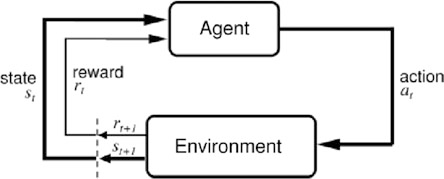
\includegraphics{pics/rl_agent_loop.png}	\caption{iterative Interaktion zwischen Agent und Environment, Abbildung entnommen aus \cite[S. 2]{Sewak2019}}
	\label{fig:rl_agent_loop}
\end{figure}

Ferner bringt das Aufstellen einer Rewardfunktion Schwierigkeiten mit sich, da sie versucht eine sinnvolle Vorhersage für die Bewertungen eines Zustandes zu ermitteln. Probleme können dabei beispielsweise darin liegen, dass Belohnungen womöglich erst im zukünftigen Verlauf zu Trage treten können oder dass sie zum gegenwärtigen Zeitpunkt schlichtweg noch ungewiss sind. Mögliche Lösungen hierfür sehen allerdings je nach Anwendungsdomäne verschieden aus \cite[S. 4-7]{Sewak2019}.

Reinforcement Learning Modelle sind als \glqq Markov Devision Process\grqq{} (MDP) anzusehen. Das hat zur Folge, dass aufgrund der zugrundeliegenden \glqq Markov Property, sowie Markov Chain\grqq{} die Wahrscheinlichkeiten für die nächstmöglichen Aktionen lediglich vom derzeitigen Zustand und nicht von weiteren vorangegangen abhhängen. Der MDP wendet diese Regeln auf den Entscheidungsprozess an, der im Fall von RL die Policy darstellt. Des Weiteren liefert der MDP die Wahrscheinlichkeiten für Zustandsübergange in der Form $P_{a}(s, s')$ an, wobei a für die mögliche Aktion, s für den aktuellen und s' für den resultierenden Zustand steht. Die Notation des entsprechenden Rewards lautet $R_{a}(s, s')$ \cite[S. 19f.]{Sewak2019}.

Weitere Begriffe, die im Kontext von RL von Bedeutung sind, sind \glqq{}Policy Evaluation\grqq{} und \glqq{}Policy Iteration\grqq{}. Erstere steht für die geschätzte Bewertung des Zustandes. Letztere beschreibt einen Iteration Prozess mit dem Ziel, dass die Policy konvergiert \cite[S. 27]{Sewak2019}.

\subsection{Zusammenspiel von MCTS und NN}
AlphaGoZero und AlphaZero basieren auf der Kombination des MCTS und des NN. Dabei gibt es zwei Schnittstellen zwischen diesen beiden Komponenten. 
Erstere liegt in der bereits erwähnten Bewertung von Blattknoten. Der MCTS durchläuft keinen simulierten Spielablauf, sondern überlässt die Evaluation des Knotens dem NN und arbeitet mit den zurückgegeben Daten weiter. Dies spiegelt die policy evaluation wider \cite{Silver2017}.

Eine weitere Verzweigung von MCTS und NN tritt bei dem Update der Parameter des NN auf. Das NN ermittelt zu jedem Spielstand die möglichen Züge und gibt deren Gewinnwahrscheinlichkeit, sowie die Wahrscheinlichkeit für die Auswahl des Zuges an. Für die Aktualisierung der Parameter werden die genannten Werte dahingehend angepasst, dass sie den im MCTS ermittelten Werten entsprechend beziehungsweise sich diesen annähern. Eine Anpassung in diese Richtung ist sinnvoll, da die Daten im MCTS als deutlich genauer gelten. Dieser Vorgang entspricht der policy improvement \cite{Silver2017}.

\newpage
% ----------------------------------------------------------------------------------
% Kapitel: Implementierung/Umsetzung
% ----------------------------------------------------------------------------------
\section{Implementierung}

\subsection{Monte Carlo Tree Search}
Um den MCTS für Reversi zu realisieren wurden die Klassen MCTS und Node angelegt. Letztere enhält zwei überladene Konstruktoren zum Anlegen von Wurzel- und Kindknoten. Ein Node enthält zusätzliche Attribute. Sowohl der Elternknoten als auch eine ArrayList vom Typ Node, die die direkten Kinder enthält, werden abgespeichert. Die Anzahl, wie oft ein Knoten besucht wurde, wird in der Variable \texttt{numVisited} hinterlegt. Außerdem gespeichert wird das Ergebnis eines simulierten Spieldurchlaufs in \texttt{simulationReward}. Da der aktuelle Spielzustand durch das Environment, das ebenfalls die derzeitige Repräsentation des Playgrounds beinhaltet, definiert ist, wird dies ebenfalls im Node hinterlegt. Des Weiteren wird in dem Attribut \texttt{nextPlayer} festgehalten, welcher Spieler als Nächstes an der Reihe ist.

Es gibt einen überladenen Konstruktor, der einerseits für das Anlegen einer neuen Wurzel und andererseits für das Erzeugen eines neuen Kinderknotens zuständig ist. Bei der Instanziierung durch die Konstruktoren werden sinnvolle initiale Werte vergeben. numVisited und simulationReward werden auf 0 beziehungsweise 0.0 gesetzt. Für den Wurzelknoten gilt, dass er keinen Parent besitzt, für alle weiteren Knoten wird der Parent übergeben und gesetzt. Die Children werden zunächst durch eine leere Liste initialisiert. Der \texttt{nextPlayer} wird ebenfalls übergeben und gesetzt. Außerdem zu erwähnen ist die Methode \texttt{calculateUCT()}, die den Upper Confidence Bound applied to Trees (UCT) für einen Knoten berechnet. Sie ermittelt zunächst die Exploitation-Komponente, indem sie den simulationReward durch die Anzahl an Besuchen dividiert. Die Exploration berechnet sich aus dem Verhältnis, wie oft der Parent besucht wurde, geteilt durch den inkrementierten Wert, wie oft der aktuelle Knoten besucht wurde. Aus dem Quotient wird anschließend die Wurzel gezogen. Um den Kompromiss zwischen diesen beiden Komponenten zu kontrollieren, wird die Exploration mit der A-priori-Wahrscheinlichkeit für einen Zug multipliziert. Diese wird im neuralen Netz trainiert.

Hinsichtlich der Klasse MCTS ist festzuhalten, dass diese in der Klasse Agent über den Konstruktoraufruf instanziiert wird. Dieser verlangt das Environment und den Player als Übergabeparameter und legt daraufhin einen neuen Wurzelknoten an, sowie eine leere ArrayList vom Typ Node, die die Blattknoten beinhaltet, die im späteren Verlauf simuliert werden müssen. Für die Simulation muss beachtet werden, dass das Environment geklont und somit eine tiefe Kopie erzeugt werden muss, damit der tatsächliche Spielzustand nicht unbeabsichtigt manipuliert wird. Dabei ist festzuhalten, dass dies zweimal stattfindet. Einmal, wenn ein neuer Baum aufgebaut wird, somit erhält der neue Wurzelknoten und ebenfalls jedes seiner Kinder jeweils einen eigenen Klon. Für die Kinderknoten gilt, dass diese ihre Environment-Instanz an ihre Kinder weitergeben und diese somit innerhalb derselben Instanz agieren. Um den MCTS zu starten, wird die Methode \texttt{searchBestTurn()} aufgerufen. Diese expandiert zunächst den Wurzelknoten, indem sie alle im aktuellen Zustand möglichen validen Züge ermittelt und durch diese iteriert. Die Methode \texttt{getPossibleTurns()} gibt diese zurück. Sie iteriert über das gesamte Spielfeld und prüft dabei mithilfe der Methode \texttt{validateTurnPhase1()} im Environment, an welcher Stelle ein gültiger Zug gemacht werden kann. Für jeden dieser Züge wird in \texttt{expand()} der Kinderknoten angelegt, sowie als unbesuchter Blattknoten abspeichert. Außerdem wird ermittelt, welcher Spieler als Nächster einen Zug machen darf und der simulierte derzeitige Spielzustand anhand des Zuges aktualisiert. Nachdem ein Knoten expandiert wurde, wird er aus der Liste der Blattknoten wieder entfernt.
Daraufhin werden die unbesuchten Blattknoten, die am Anfang den Kinderknoten der Wurzel entsprechen, in der Methode \texttt{traverse()} durchlaufen. Dabei wird in jedem dieser eine Simulation gestartet, die einen Spielverlauf bis zum Spielende anhand zufällig ausgewählter möglicher Züge durchspielt. 

Mithilfe der Funktion \texttt{simulate()} erfolgt die Simulation eines Spiels. Ein Zufallszug wird durch eine Instanz der Java-Klasse Random generiert. Hierbei wird ein zufälliger Integer erzeugt, der durch eine Modulo-Operation auf den Größenbereich abgestimmt wird, der dem der Anzahl der möglichen Züge entspricht. Die resultierende Zahl gibt den auszuwählenden Zug innerhalb der ArrayList an.

Wenn keine weiteren validen Folgezüge ermittelt werden können, bedeutet das das Spielende und der Reward für die Spielausgang wird anhand der Funktion \texttt{rewardGameState()} berechnet. Diese erhält als Parameter das Environment, sowie den Spieler, für den der Reward kalkuliert werden soll. Indem der gesamte Playground durchlaufen und gezählt wird, wie viele Steine vom übergebenen Spieler enthalten sind, errechnet sich die Bewertung des Spiels. Abschließend werden die Werte für Anzahl Besuche und Reward ebenfalls im Wurzelknoten aktualisiert.

Nach Abschluss der Simulation wird der Reward zurückgegeben. Daraufhin wird in \texttt{traverse()} die Backpropagation der Ergebnisse durchgeführt, indem iterativ vom aktuellen Knoten bis hoch zur Wurzel die Anzahl an Besuchen inkrementiert und der Reward entsprechend erhöht wird.

\newpage

% ----------------------------------------------------------------------------------
% Kapitel: Allgemeine Informationen/Organisation
% ----------------------------------------------------------------------------------
\section{Organisation}

\subsection{Team und Aufgabenverteilung}
% Beschreiben Sie in diesem Abschnitt Ihr Team. Welche Person hat welche Aufgaben wahrgenommen, wie wurden
% Aufgaben aufgeteilt und wie wurde kommuniziert, etc.
Als Vierer-Team bestand unsere Gruppe aus Simon Hofmeister, Nadiia Matsko, Monika Silber und Simon Wasserburger. Anzumerken ist, dass Simona Hofmeister und Simon Wasserburger bereits im Bachelorkurs Erfahrung mit dem Implementieren einer künstlichen Intelligenz für Reversi sammeln konnten. Aus diesen Gründen griffen wir für den Aufbau dieses Projektes auf das Grundgerüst des bereits im Bachelorkurs erstellen Programms von Simon Hofmeister zurück, der dieses entsprechend an die Anforderungen des vorliegenden Projektes anpasste.

Die weiteren Komponenten verteilten wir wie folgt:
Simon Hofmeister: Aufsetzen des Grundgerüsts, Implementierung des NN
Nadiia Matsko: Implementierung des NN, Verfassen des Kapitels Einleitung in der Dokumentation
Monika Silber: Implementierung des MCTS, Verfassen der Kapitel theoretischen Grundlagen des MCTS und Organisation in der Dokumentation
Simon Wasserburger: Implementierung des MCTS, Erstellen der Grafiken für MCTS, Code-Refactoring (Grundgerüst)
%TODO Ergänzungen

Hinsichtlich des Aufwands für diese Aufgaben ergab sich für die einzelnen Teammitglieder folgende Verteilung:
%TODO Aufdröselung in Recherche, Implementierung, Doku und Orga

\subsection{Kommunikation}
Die virtuelle Kommunikation fand hauptsächlich in unserer WhatsApp-Gruppe statt, wo wir einander auf Problemstellen aufmerksam machten, Lösungsansätze diskutierten, einander über Fortschritte informierten und Treffen ausmachten. Ebenfalls konnte durch Commits im Repository die Arbeit der Teamkollegen und entsprechend der Projektfortschritt verfolgt werden. Daneben verfügten wir über ein Trello-Board, in dem wir Aufgaben planten, dokumentierten und zuwiesen. In gemeinsamen Treffen besprachen und ergänzten wir dabei die offenen Punkte und kontrollierten den Projektablauf. 

In den persönlichen Treffen, in denen meist alle Teammitglieder anwesend waren, konnten wir alle offenen Punkte konkretisieren und ausführlich diskutieren. Wir erarbeiteten gemeinsame Lösungsstrategien und halfen einander bei Verständnisproblemen. Abschließend trafen wir Absprachen zum weiteren Vorgehen, sowie zur Aufgabenverteilung.

\subsection{Versionskontrolle}
Als Versionskontrollsystem stand ein Gitlab-Repository der OTHR zur Verfügung. Zum Abrufen und Bearbeiten dessen wurde GitHub Desktop als GUI verwendet.
%TODO welche GUI/CLI?

Hinsichtlich Implementierung der Komponenten wurden eigene Branches angelegt, die vom master-Branch geklont und nach Fertigstellung entsprechend dort wieder gemergt wurden. Dabei ergaben sich eigene Branches für den MCTS, das NN, sowie für den Prozess des Refactoring des ursprünglichen Codes. Die finale und alle Bestandteile umfassende Version befindet sich folglich im master-Branch.

\subsection{OS, IDE und Programmiersprache}
%TODO OS
Als Entwicklungsumgebung wurde IntelliJ IDEA\footnote{https://www.jetbrains.com/de-de/idea/} von JetBrains genutzt. Java wurde als Programmiersprache zur Impelementierung des Projektes verwendet. Zur Erstellung des Programms kam maven\footnote{https://maven.apache.org/} als Build-Management-Tool zum Einsatz.

\subsection{Testumgebungen}

\subsection{Projekt-Dokumentation}

\newpage
% ----------------------------------------------------------------------------------
% Kapitel: Fazit
% ----------------------------------------------------------------------------------
\section{Fazit}
% Beschreiben Sie in diesem Abschnitt u.a.\ was Ihnen an diesem Fach gefallen hat und welche
% Verbesserungsvorschläge Sie für künftige Veranstaltungen haben. Was konnten Sie dazulernen, in welchen
% Bereichen haben Sie sich verbessert. Welche Problemsituationen gab es während der Projekterstellung, wie
% sind Sie diese angegangen und wie haben Sie diese gelöst. Was haben Sie evtl.\ vermisst.

\pagebreak

%\newpage
% ----------------------------------------------------------------------------------
% Kleine Einführung in LaTeX-Elemente
% ----------------------------------------------------------------------------------
% \section{\LaTeX-Elemente}
% Dieser Abschnitt soll nicht Bestandteil des Projektberichtes sein, sondern beinhaltet lediglich einige
% Informationen über \LaTeX-Distributionen, Editoren und \LaTeX-Elemente, die Ihnen beim Einstieg in das
% \LaTeX-Textsatzsystem helfen sollen.

% \subsection{\LaTeX-Distributionen nach Betriebssystemen}

% \subsubsection{\LaTeX-Distributionen}

% Folgende Haupt-\LaTeX-Distributionen stehen Ihnen zur Verfügung:
% \begin{itemize}
%  \item Windows:\quad \texttt{MiKTeX}\quad Webseite:\quad\url{http://www.miktex.org}
%  \item Linux/Unix:\quad \texttt{TeX Live}\quad Webseite:\quad\url{http://tug.org/texlive/}
%  \item Mac OS:\quad \texttt{MacTeX}\quad Webseite:\quad\url{http://www.tug.org/mactex/}
% \end{itemize}

% \subsubsection{\LaTeX-Editoren}
% Auf folgenden Webseiten können Sie einige hilfreiche \LaTeX-Editoren finden:
% \begin{itemize}
%  \item Windows/Linux/Mac OS: \url{http://www.xm1math.net/texmaker/}
%  \item Windiws: \url{http://www.texniccenter.org/}
%  \item Mac OS: \url{http://pages.uoregon.edu/koch/texshop/}
% \end{itemize}

%Falls bei den oben genannten Editoren kein passender vorhanden war, findet sich auf Wikipedia eine  %Zusammenstellung vieler weiterer \LaTeX-Editoren:\\[1em]
%\hspace*{3cm}\url{https://en.wikipedia.org/wiki/Comparison_of_TeX_editors}


%\subsection{Unterabschnitt}
%Zum Einfügen eines Bildes, siehe Abbildung \ref{fig:reversi01}, wird die
% \textit{minipage}-Umgebung 
%genutzt, da die Bilder so gut positioniert werden können.

%\vspace{1em}
%\begin{minipage}{\linewidth}
%	\centering
%	\includegraphics[width=0.6\linewidth]{pics/gamefield01.png}
%	\captionof{figure}[Spielfeld 01]{Unbespieltes Spielfeld\footnotemark }
%	\label{fig:reversi01}
%\end{minipage}
%\footnotetext{Diesem Spielfeld wurden noch keine Spieler zugewiesen (daher die
% dunklen Spielsteine)}

%Nachdem das Spiel gestartet wurde und beiden Spielphasen durchlaufen wurden, siegt
% schließlich der %Spieler mit der Farbe rot.

%\vspace{1em}
%\begin{minipage}{\linewidth}
%	\centering
%	\includegraphics[width=0.6\linewidth]{pics/gamefield02.png}
%	\captionof{figure}[Spielfeld 02]{Finales Spielfeld\footnotemark }
%	\label{fig:reversi2}
%\end{minipage}
%\footnotetext{Das Spielfeld nach der Zug- und Bombenphase. Spieler rot gewinnt
% eindeutig.}

%\subsection{Tabellen}
%In diesem Abschnitt wird eine Tabelle (siehe Tabelle \ref{tab:beispiel}) dargestellt.

%\vspace{1em}
%\begin{table}[!h]
%	\centering
%	\begin{tabular}{|l|l|l|}
%		\hline
%		\textbf{Name} & \textbf{Name} & \textbf{Name}\\
%		\hline
%		1 & 2 & 3\\
%		\hline
%		4 & 5 & 6\\
%		\hline
%		7 & 8 & 9\\
%		\hline
%	\end{tabular}
%	\caption{Beispieltabelle}
%	\label{tab:beispiel}
%\end{table}


%\subsection{Auflistung}
%Für Auflistungen wird die \textit{enumerate}- oder \textit{itemize}-Umgebung genutzt.
%
%\begin{itemize}
%	\item Nur
%	\item ein
%	\item Beispiel.
%\end{itemize}
%
%\subsection{Listings}
%Zuletzt ein Beispiel für ein Listing, in dem Quellcode eingebunden werden kann, siehe Listing \ref{lst:arduino}.
%
%\vspace{1em}
%\begin{lstlisting}[caption=Arduino Beispielprogramm, label=lst:arduino]
%int ledPin = 13;
%void setup() {
%    pinMode(ledPin, OUTPUT);
%}
%void loop() {
%    digitalWrite(ledPin, HIGH);
%    delay(500);
%    digitalWrite(ledPin, LOW);
%    delay(500);
%}
%\end{lstlisting}
%
%\subsection{Tipps}
%Die Quellen befinden sich in der Datei \textit{quellen.bib}. Eine Buch- und eine Online-Quelle sind beispielhaft eingefügt. [Vgl. \cite{buch}, \cite{online}]
%
%\pagebreak

% ----------------------------------------------------------------------------------------------------------
% Literatur
% ----------------------------------------------------------------------------------------------------------
\renewcommand\refname{Literatur}
\bibliographystyle{alpha}
\bibliography{literatur}

%\printbibliography

\pagebreak

% ----------------------------------------------------------------------------------------------------------
% Anhang
% ----------------------------------------------------------------------------------------------------------
\pagenumbering{Roman}
\setcounter{page}{1}
%\lhead{Anhang \thesection}

\begin{appendix}
\section*{Anhang}
%\phantomsection
\addcontentsline{toc}{section}{Anhang}
\addtocontents{toc}{\vspace{-0.5em}}

\end{appendix}

\end{document}